 
\section{Validation}
\label{sec:validation}


%% \begin{figure}[h]
%%  \begin{center}
%%   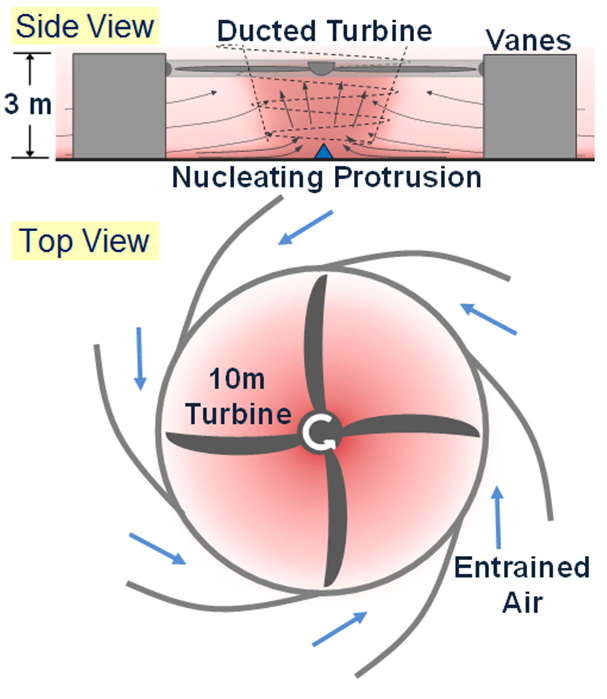
\includegraphics[width=.5\linewidth]{fig/power_generation.png}
%%    \caption{The Sov facility, showing the vanes, rotor and anchoring
%%    protrusion, as well as the buoyancy-driven vortex used to drive the
%%    turbine.}
%%    \label{facility}
%%   \end{center}
%% \end{figure}

The simulations are designed to both mimic the notional SoV experimental
facility as well as identify optimal configurations for future
designs. The general system configuration is depicted in Figure
\ref{facility}. 

Notice several important components of this device. First, ``vanes''
along the sides of the apparatus, designed to entrain outside air and
impart angular momentum. It is not known what configuration and design
of these vanes will lead to optimal dust-devil generation. Thus, these
vanes may have various configurations, varying in the number used, the
length, height, angle of attack. The vanes may also be straight, or
curved.  Next, the ducted turbine above the flow is also a critical design
component. This turbine is designed to extract energy from the flow,
without distrupting/destroying the vortex. Finally, it is desirable to
economically optimize the entire configuration scale by considering both
the power generation, cost of materials, difficulty and expense of
maintainance, etc. 

The model inputs consistitute a very large component (arguably, the
largest source) of the uncertainty in this problem, for both the
laboratory and outdoor test cases. For brevity, we consider here only
the laboratory cases. 

  \begin{figure}[!htb]
    \begin{center}
     \includegraphics[width = 12 cm]{figs/lab_setup}
     \caption{The laboratory set-up.}
     \label{lab}
    \end{center}
  \end{figure}

The experimental laboratory has numerous objects
in the immediate vicinity (see figure \ref{lab}) that may
obstruct/manipulate the flow. These objects may be moved or removed
during PIV data gathering. The laboratory simulation uses adiabatic side
walls as a boundary condition. It is unclear how much of an impact this
may have on the simulation. It is also unclear if this is a realistic
boundary condition. 

While no sensitivity analysis has been performed, it is likely that the
largest uncertainty in the laboratory simulation is a result of the
ventilation. This statement can be made because it was observed that the
heated plate on the bottom of the laboratory generated enough heat that
the room temperature began to rise significantly (30+ degrees
Celsius). This also greatly impacted the SoV performance, as the ground
to air thermal gradient drives the vortex. The laboratory uses cooling
in order to maintain temperature. They utilize two inlet HVAC ducts into
the room. While efforts have been made to characterize the level of
ventillation being used, these numbers come with non-trivial
uncertainties attached. As an example, a personal communication with one
of our experimental colleagues, 

``One vent runs continuously at 15 C with a flow rate of about 1
$m^3$/s (4-6 m/s with an approximate area of 0.2 $m^2$).''
Already, the inflow rate has a 50\% uncertainty in velocity
attached. Furthermore, while the area of the vents are given, the the
precise height and width are not. Thus, while our simulation uses square
vents, this may be inaccurate. 
It was also stated that, ``The other vent kicks on only if the
room gets about 28 degrees C.'' This statement has uncertainty attached to the
temperature at which the venting begins. Finally, ``The exit air is just
what ever leaves through/around the doors as we've blocked off all of
the out ducts.'' This also presents a challenge, as it is unclear (for
validation purposes) where one should expect the outflow to
go. \footnote{\normalsize Author note: This story related here not as a comment on
our collaborators. Rather, this is presented as an example of the challenges
and uncertainties that presently exist in this numerical investigation.}

We impose Dirichlet boundary conditions to establish a constant inflow
condition of cool air at the rates proscribed by our
collaborators. Unfortunately, we have found that the using inflow rates
consistent with the lower bound of those estimates result in an
unrealistic heating of the room, while inflow conditions at the high end
result in velocity profiles that exceed the laboratory measurements. In
other words, our simulations appear to be sensitive to the choice of
inflow rate, and it is likely that the laboratory is run where one of
the vents is operating intermittently. 

The initial conditions in both the laboratory and the outdoor
tests are highly uncertain. The dimensions of the laboratory are
(it is presumed) measured with a high degree of confidence, however, the
initial temperature 
in the room is not closely measured, and may vary as a function of
time or across tests. We note however, that the solutions from the simulations are
generally stationary in time, and consistent results are gathered from several
simulations with different initial conditions. Therefore, it does not
appear that the initial conditions in the room in terms of the ambient
velocity or temperature field are a large source of uncertainty in the
laboratory.

\subsection{Model Calibration}

%
% viscosity calibrated
% 


\subsection{Challenges}

Several phases of research must be conducted in order to develop robust
and reliable predictive simulation capability. First, the simulations
must be validated against existing experimental data generated from the
laboratory apparatus. These data were taken using particle image
velocimetery (PIV), often not without non-trivial error in measurement and
sampling. Finally, as mentioned previously, the measurements for the
cooling, geometry of the room, etc. are rough, and almost certainly
possess non-trivial uncertainties/errors. As a result, this is already a
difficult validation scenario. 

The validation challenge is compounded by the fact that very little is
known about the uncertainties in the observation data. PIV is a
non-intrusive technique, but it does rely upon large sample sizes in
order to generate reliable statistics. While several hundred PIV
snapshots are available, no quantified uncertainties for the averaged fields
presently exist.  

In addition, only velocity measurements are available. Several
potentially important quantities of interest, such as the pressure field
or the temperature, have not been measured, and cannot then be used for
the purposes of validation. This presents a risk that our 
simulations might generate acceptable velocity fields, but that a
significant source of error may exist in unobserved QoIs, and would not
be detected in our present validation regime. 

Furthermore, the model form in use is known to be imperfect. 
Model inadequacy may play a significant role in both the validation
scenarios described below, as well as (more chillingly) in the
additional regimes that the models will be used in a predictive
capacity. 

\subsection{Model Validation}
Our initial focus has therefore moved to a validation study to ensure that the
output of the numerical simulation agrees with the experimental
measurements. The flows are qualitatively similar, with a vortex forming
in the center of in both cases, but the degree to which each matches
each other is unclear and must be characterized. 

In particular, we have implemented a simulation designed
to closely mimic the 30 degree vane experimental setup. The outputs of
the simulation (velocity field, temperatures, etc. ) are then compared
to available experimental data, which at this time is principally the
velocity field taken by PIV measurements at a variety of time frames
near the center of the SoV. This ``high-cost'' simulation resolves
the SoV large-scale structure, as well as the turning vanes
nearby. Comparisons must be made between the:
\begin{itemize}
 \item Azimuthal Velocity as a function of radius from center of the Sov
 \item Azimuthal Velocity as a function of the height at different
       points in the SoV
 \item Vertical Velocity as a function of radius from center of the Sov
 \item Vertical Velocity as a function of the height at different
       points in the SoV
\end{itemize}
As noted above, this is an extremely limited set of comparisons. 

%
% hybrid (embedded model)
%
Further validation cases are required. We are now in a position to perform
a validation of the embedded vane model. As described previously, this
uses the same turbulence models, but now without resolving the turning
vanes. Instead of resolving the vanes, for a region in the flow, the
velocity field is forced in a manner similar to as if the fluid was
moving through the turning vanes. While direct comparisons between this
model and the experimental data can be (and will be) made, a comparison between this
``low-cost'' (in terms of computation and mesh requirements) simulation
and is useful for several reasons. It permits directly comparing the effect of
the simple, low cost, turning vane model against the higher resolution
modeling (essentially this permits a validation of an embedded
model). Furthermore, it allows us to observe a much richer set of
possible changes in the state space than in the experiment, which is
constrained to only velocity measurements. 

%
% 7) An assessment of what further concerns might remain after (5) and
%   (6) regarding the applicability of the model for the purpose of the
%   calculations.
%
\section{Further Concerns}

% the fucking turbine too...
Our goal is to eventually extract energy from the SoV, which at this
time is envisioned coming from a turbine placed over the vanes. It will
be very difficult to get accurate PIV measurements from the apparatus in
the laboratory, and once again the simulations will be essential in
driving the experimental optimization and design of the SoV. Thus, 
this adds another significant validation case, with new, significant,
challenges in modeling the turbines. This is in essence a new embedded
submodel that we will add after validation of the initial configuration
is completed. 

In order for these simulations to be generally useful, after they are 
validated against existing experimental data and high fidelity
simulations, they will be used to explore regimes and scales where no
experimental measurements presently exist. Characterizing the
uncertainty of predictions resulting from extrapolation is a critical
component in enabling reliable assessments of field performance of the
SoV, as it will guide the commercialization strategy of the product.

% scaling analysis
These new simulations at different conditions will be performed in order
to inform the optimal design and scale of the planned two and five meter
SoV prototypes, to be installed in Arizona. This study will inform the
design based on the scaling of the velocity field and anticipated energy
generation. Furthermore, insights may be gathered on the dyamics of
these flows, which could lead to fundamental advances in the physics of
fluid dynamics, dust devils, and other coherent structures with vortex 
dynamics\cite{Mullen1977181,smithleslie,kanak}. 

% this might be junk
Determining the optimal design of these systems will involve parameter
sweeps over a large space of possible configurations. These simulatons
are expensive, and so while accuracy is important, where possible,
models will be developed in order to simplify the mesh (memory) and
computational requirements. For instance, the previous ``low-cost'' vane
 method, which replaces the turning
vanes with a model, improved runtime by a factor of twenty-four, due to
the greatly decreased mesh resolution requirements near the vane
trailing edges. These models, if they prove to be robust after
validation testing, will be
invaluable tools in effective computer aided design and simulation of
this new technology.  

